\documentclass[9pt]{IEEEtran}

\usepackage[english]{babel}
\usepackage{subcaption}
\usepackage{graphicx}
\usepackage{epstopdf}
\usepackage{fancyhdr}
\usepackage{amsmath}
\usepackage{amsthm}
\usepackage{amssymb}
\usepackage{url}
\usepackage{array}
\usepackage{textcomp}
\usepackage{listings}
\usepackage{hyperref}
\usepackage{xcolor}
\usepackage{colortbl}
\usepackage{float}
\usepackage{gensymb}
\usepackage{longtable}
\usepackage{supertabular}
\usepackage{multicol}
\usepackage{booktabs}

\usepackage[utf8x]{inputenc}

\usepackage[T1]{fontenc}
\usepackage{lmodern}
\input{glyphtounicode}
\pdfgentounicode=1

\graphicspath{{./figures/}}
\DeclareGraphicsExtensions{.pdf,.png,.jpg,.eps}

% correct bad hyphenation here
\hyphenation{op-tical net-works semi-conduc-tor trig-gs}
% ============================================================================================

\title{\vspace{0ex}
Project 5: Long-Term Tracking}

\author{Katarina Brešar\vspace{-4.0ex}}

% ============================================================================================

\begin{document}

\maketitle

\section{Introduction}

In this assignment we tested the performance of short-term tracker SiamFC on long-term sequences. We used precision,
recall and F-score as evaluation metrics. We then adjusted the tracker so it became a long-term tracker and again
tested it on the same sequences. We compared the results of the two trackers and analyzed the parameters.

\section{Experiments}
We first tested the performance of the short-term tracker SiamFC on a long-term sequence. The tests were performed only
on sequence car9 as there was no GPU avaliable. The results for precision, recall and F-score are shown in table~\ref{tab:siamfc_short}.
We can see that the precision is quite high, but recall is very low. So the tracker works well when the tracker is visible, but
when it dissapears from view, the tracker fails to find it again. Which was expected since the tracker is not designed for long-term tracking.
The F-score is also quite low, which is a consequence of the low recall.

\begin{table}[h!]
\centering
\begin{tabular}{|c|c|c|}
\hline
Precision & Recall & F-score \\
\hline
0.639 & 0.271 & 0.381 \\
\hline
\end{tabular}
\caption{Performance of short-term tracker SiamFC on sequence car9.}\label{tab:siamfc_short}
\end{table}

We then adjusted the tracker to make it a long-term tracker. We added a confidence threshold to decide when the tracker is not confident enough and when it should stop tracking. The results with the long-term tracker
with parameters: threshold $= 4$ and number of randomly sampled patches $=50$. With this we got the
following results for precision, recall and F-score as shown in table~\ref{tab:siamfc_long}. Comparing to the short-term
tracking results, we can see that precision is slightly lower, so there were some false positives during re-detection.
But the tracker is now able to find the target again after it dissapears from view, which is shown by the much higher
recall and consequently much higher F-score.


\begin{table}[h!]
\centering
\begin{tabular}{|c|c|c|}
\hline
Precision & Recall & F-score \\
\hline
0.600 & 0.594 & 0.597 \\
\hline
\end{tabular}
\caption{Performance of long-term tracker on sequence car9.}\label{tab:siamfc_long}
\end{table}

\subsection{Confidence score}
We defined the confidence score directly by the maximum correlation response by the network. When the correlation
drops below the threshold, the tracker assumes the target is lost and it starts re-detection. To get
the best threshold we first checked the scores outputed by the short term tracker. We saw that when the target
was lost the scores dropped to around 4 and lower. So we tested multiple thresholds and ultimately decided to use
threshold $=4$ as it gave the best F-score. In table~\ref{tab:confidence} we can see the results for different thresholds.
When it's too low the detector finds wrong objects instead of the target. Since it's satisfied with low confidence,
so it doesn't even try to find the target again, but just keeps tracking the wrong object (for example the detector
found a tree and then later the wrong car). So the recall is very low. On the other hand, when the threshold is too high,
the tracker activates re-detection too often, even when the target is still visible. So it looks for the target with
random sampling, which is not very efficient and the overlap is not very good. It also takes more time to process the frames,
which is not good for real-time tracking.

\begin{table}[h!]
\centering
\begin{tabular}{c|c|c|c|}
\hline
Threshold & Precision & Recall & F-score \\
\hline
3 & 0.647 & 0.269 & 0.380 \\
3.5 & 0.608 & 0.572 & 0.590 \\
4 & 0.600 & 0.594 & 0.597 \\
4.5 & 0.602 & 0.591 & 0.596 \\
5 & 0.601 & 0.589 & 0.595 \\
6 & 0.599 & 0.542 & 0.569 \\
\hline
\end{tabular}
\caption{Performance of long-term tracker with different confidence thresholds.}\label{tab:confidence}
\end{table} 



\subsection{Number of sampled regions}
We also tested how the number of randomly sampled patches for re-detection affects performance. While the
precision, recall and F-score stay mostly similar (all around $0.6$), the difference is in 
how many frames it takes for the target to be found again after it dissapears. How many frames are needed is shown
in table~\ref{tab:sampled_regions}. We can see that with more sampled regions the target is found faster, but not by
some significant margin. This is due to the fact that we have a uniform distribution for sampling, so it is
spread evenly across the whole image. And even with a small amount of samples, we take a similar amount of frames as we do with more.
The similar results can also be due to randomness. We do random sampling and the results can vary between different runs.

\begin{table}[h!]
\centering
\begin{tabular}{c|c}
\hline
Number of samples & Frames to re-detect \\
\hline
25 & 33 \\
50 & 31 \\
75 & 27 \\
100 & 32 \\
\hline
\end{tabular}
\caption{Number of frames required for re-detection with different numbers of sampled regions.}\label{tab:sampled_regions}
\end{table}

To get a better view of what's happening during re-detection, we also visualized the sampled regions before and after re-detection.
In figure~\ref{fig:sampled_regions} we can see that the sampled regions are spread across the whole image. When the 
target is not visible the tracker ``predicts'' the target in one of the sampled regions, far away from the actual target.
It does this since the confidence score  is low all over the image, so it's satisfied with this wrong prediction. But after
the target comes back into view, the tracker is able to find it again.

\begin{figure}[h!]
    \centering
    \begin{subfigure}[b]{0.25\textwidth}
        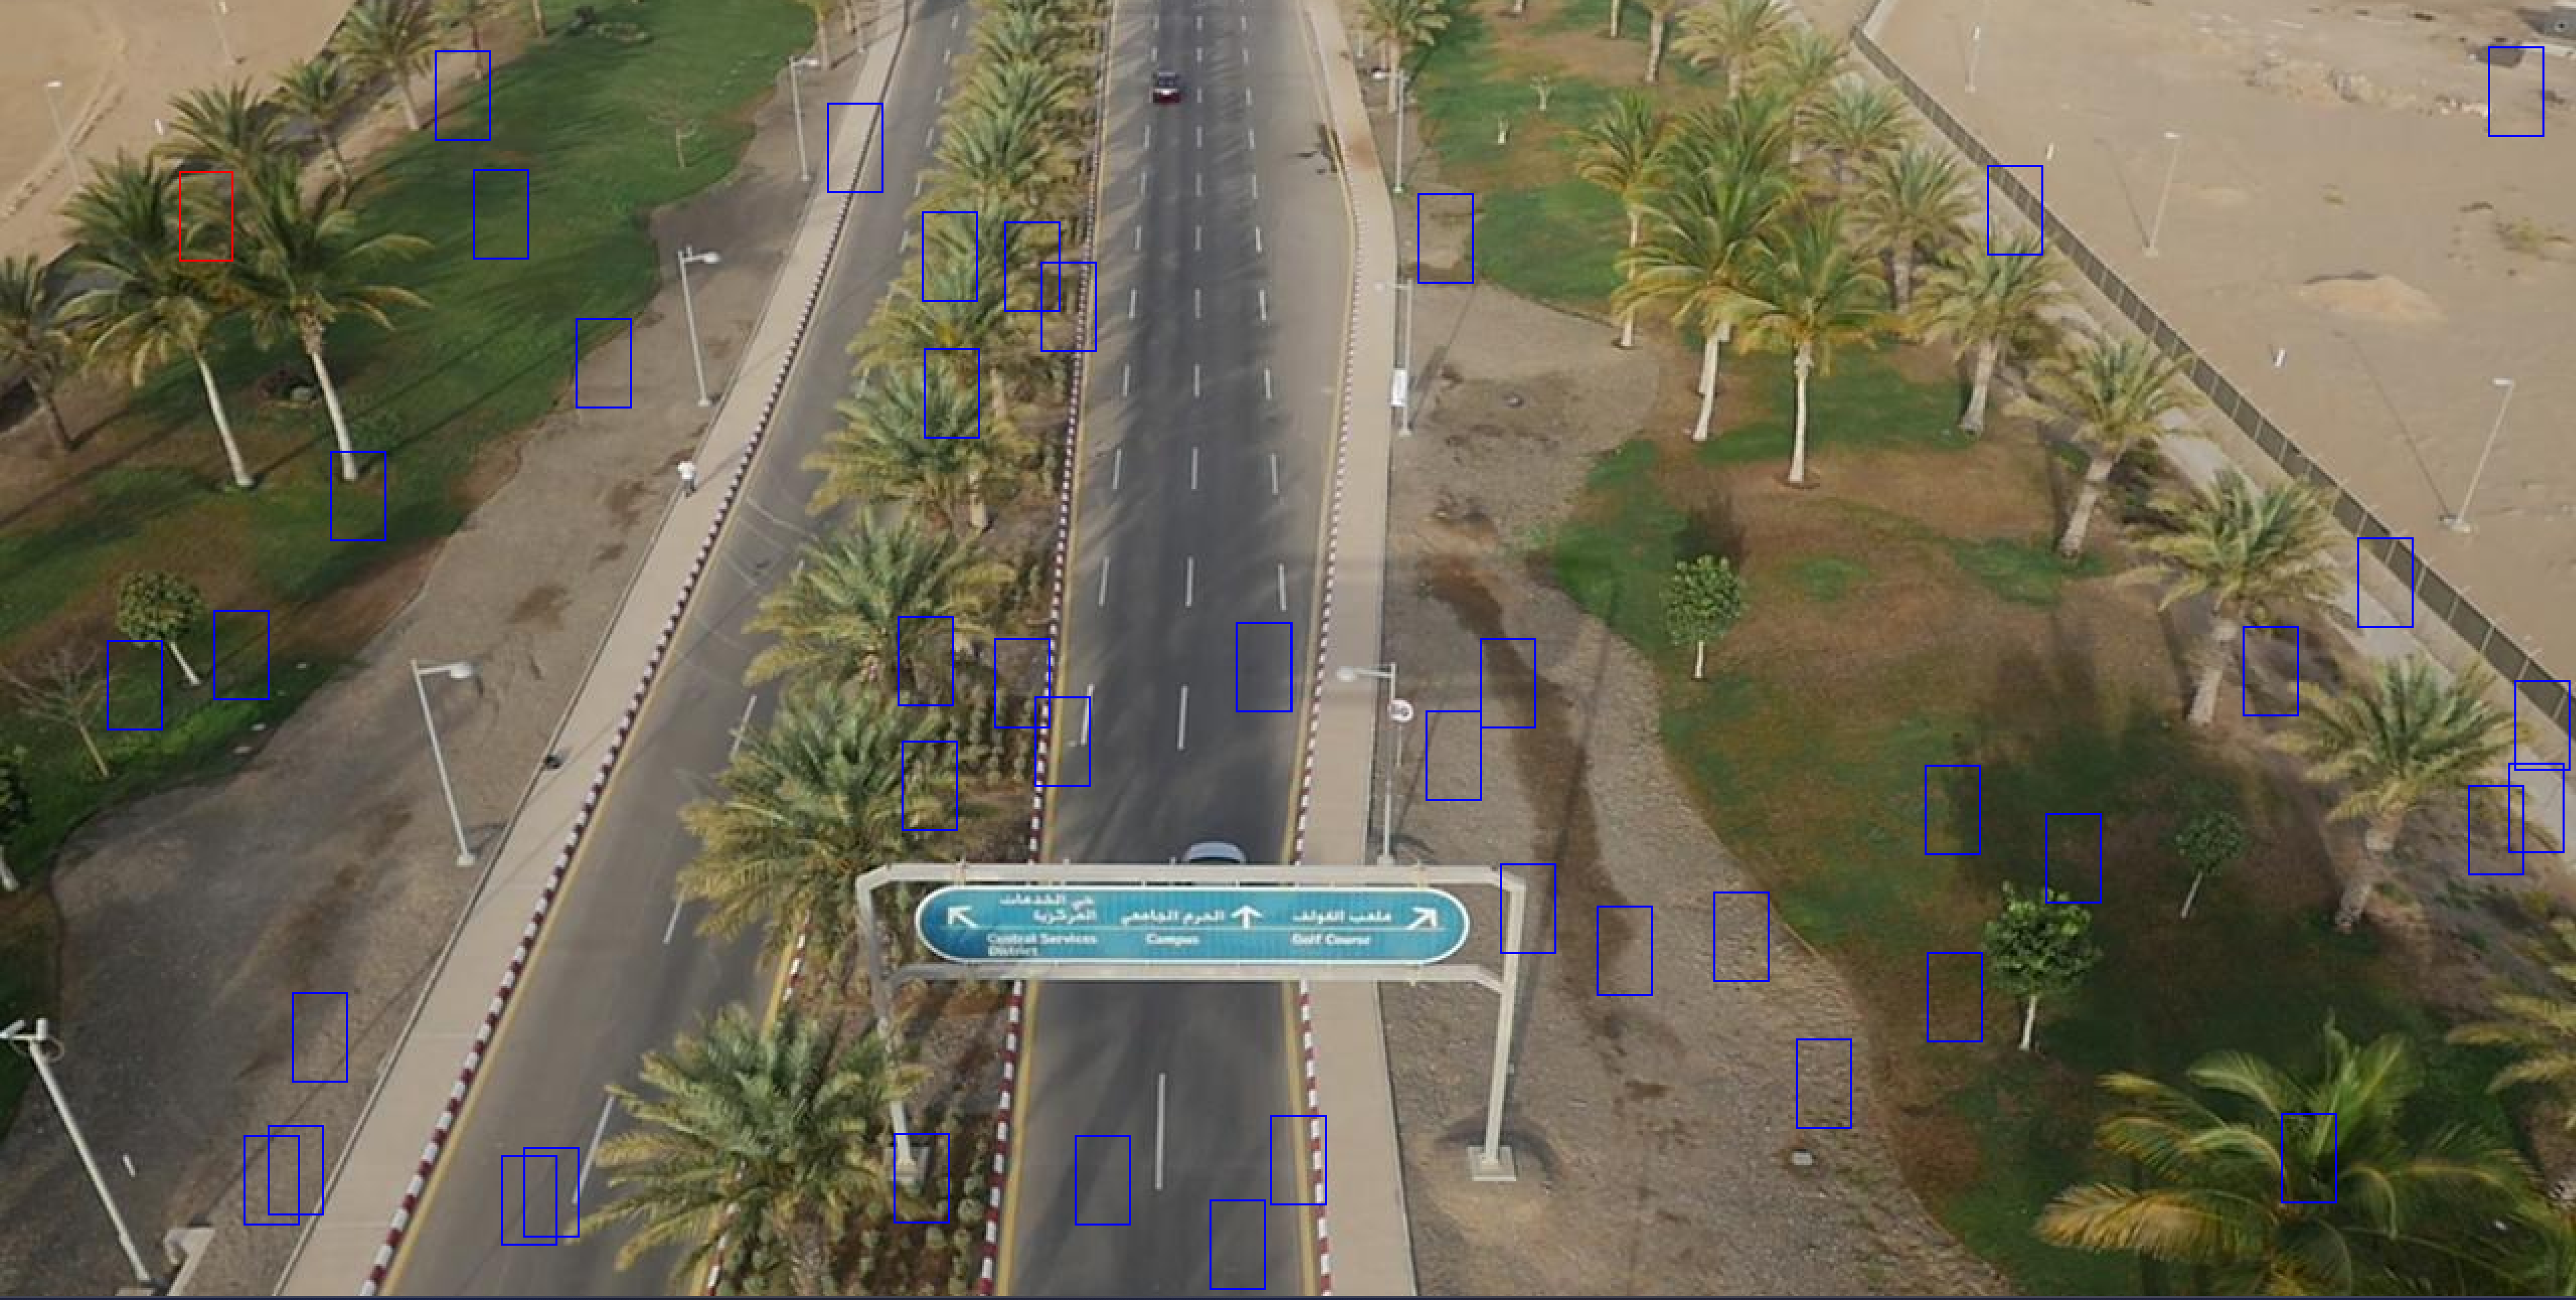
\includegraphics[width=\textwidth]{figures/uniform-pre.png}
        \caption{Sampled regions before re-detection.}
        \label{fig:sampled_before}
    \end{subfigure}
    \hfill
    \begin{subfigure}{0.25\textwidth}
        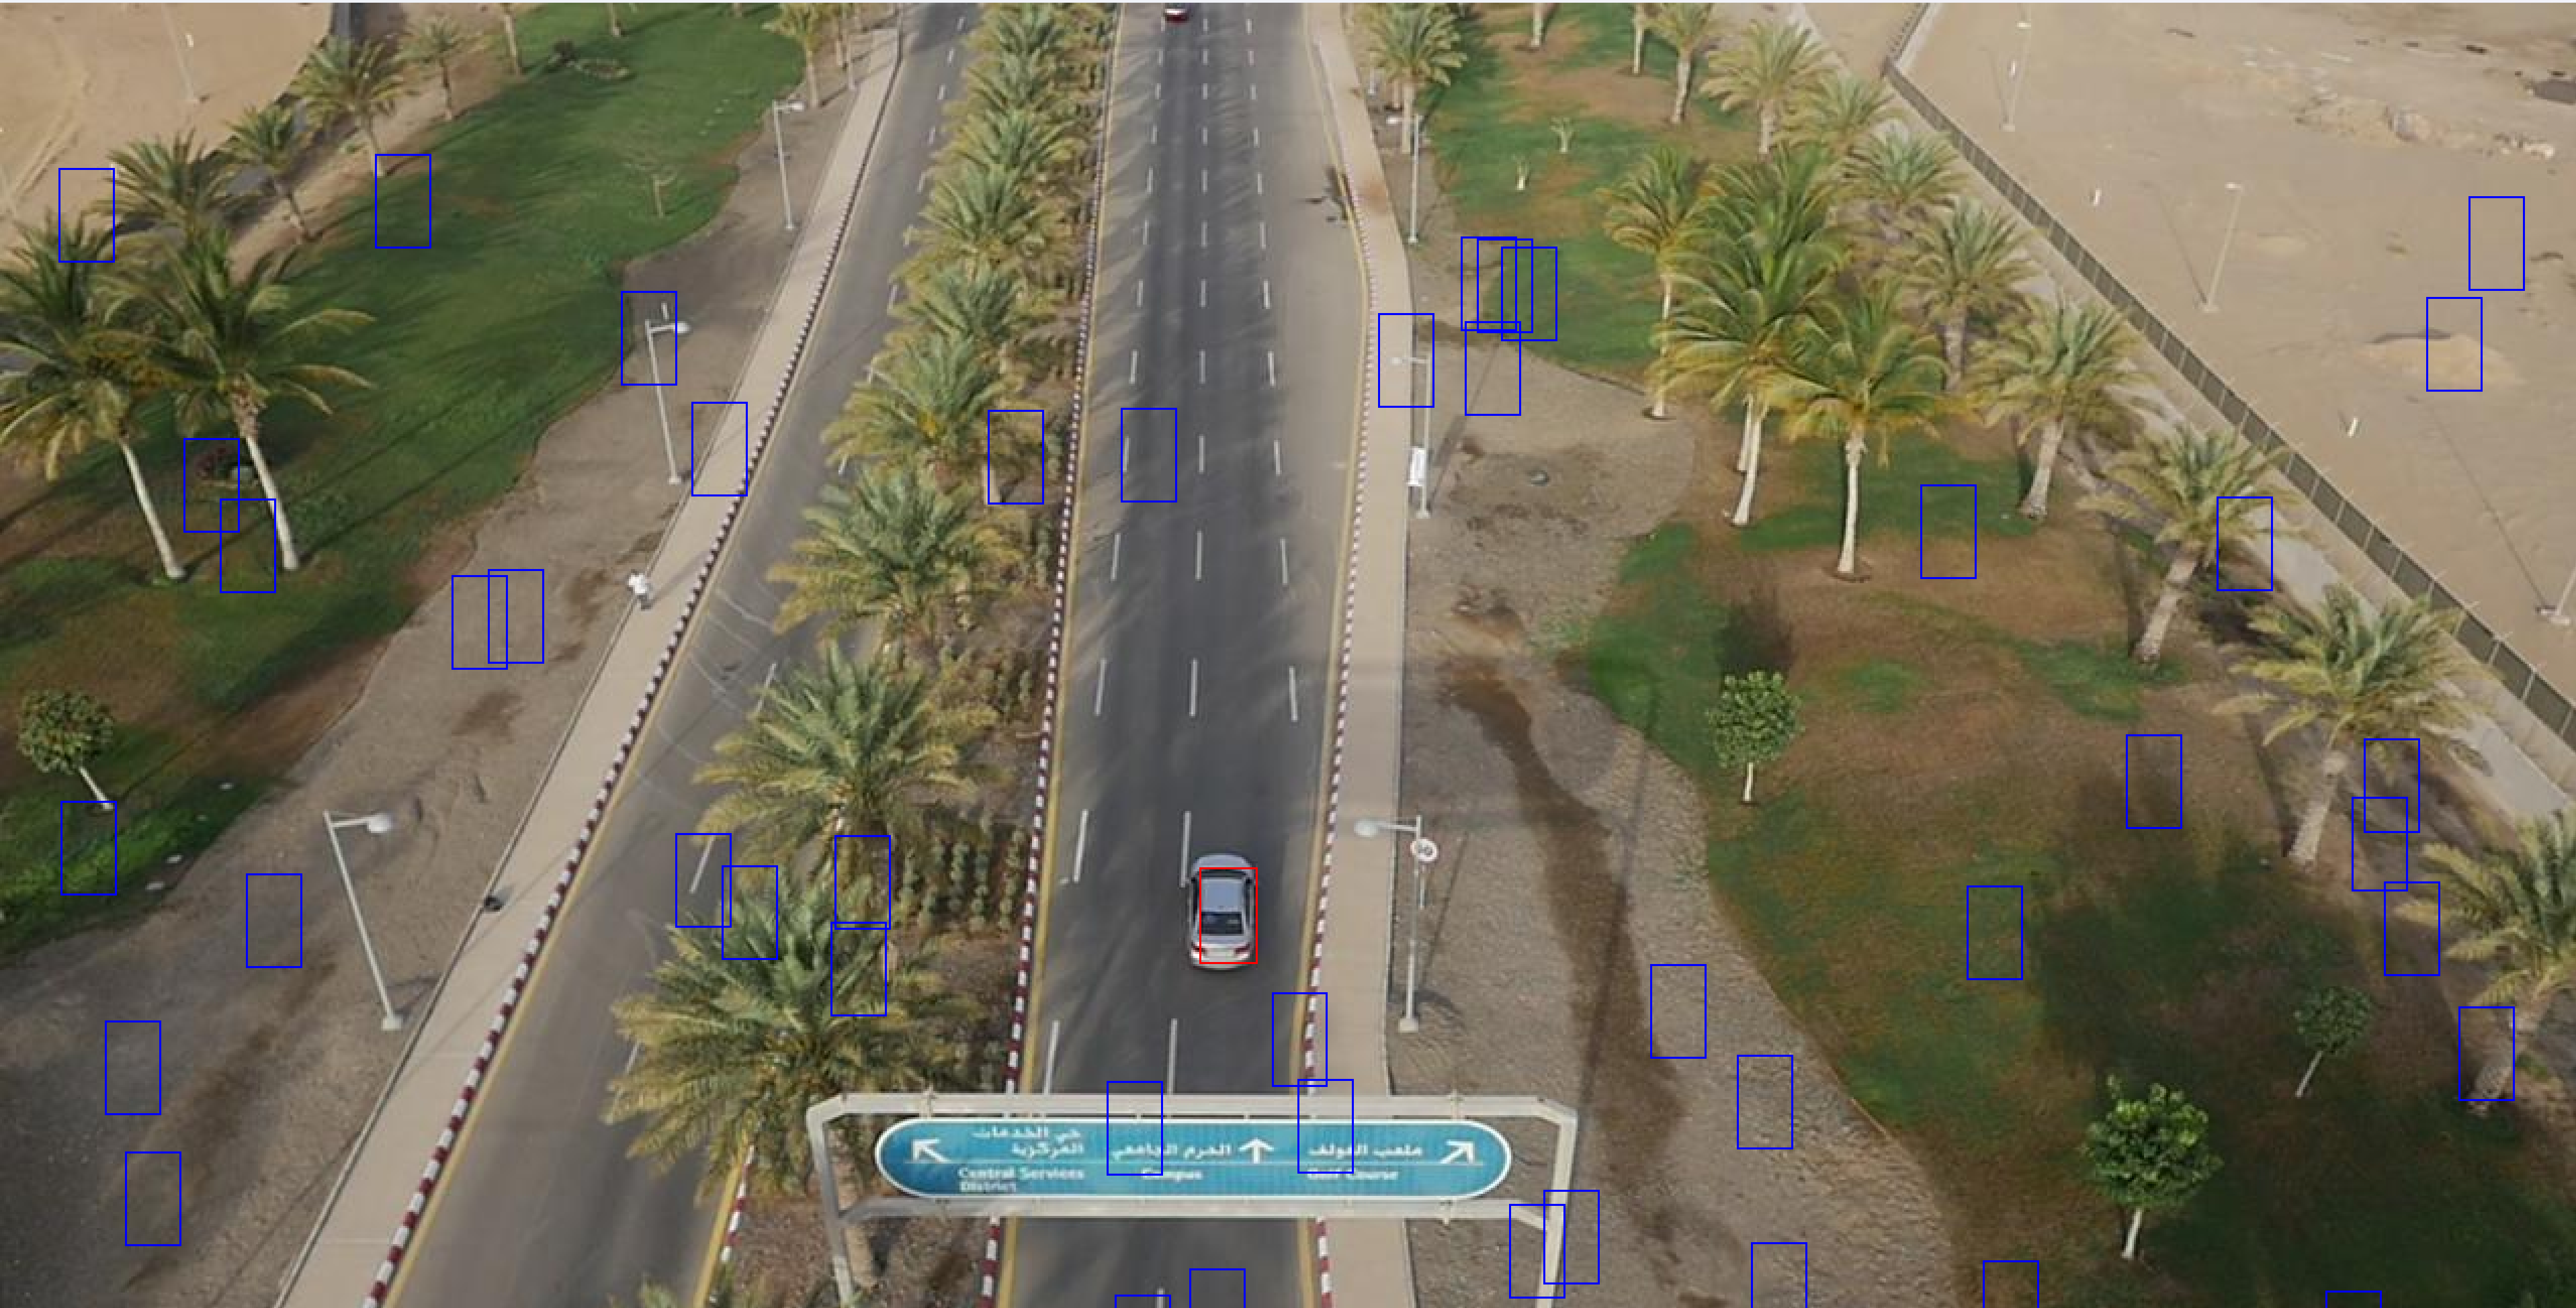
\includegraphics[width=\textwidth]{figures/uniform-post.png}
        \caption{Sampled regions after re-detection.}
        \label{fig:sampled_after}
    \end{subfigure}
    \caption{Visualization of sampled regions during re-detection. The blue rectangles are the sampled regions and the red is the prediction.}
    \label{fig:sampled_regions}
\end{figure}



\subsection{Different type of sampling}
As stated in the previous section, we used uniform sampling for re-detection. So the patches were uniformly distributed all over the image.
But we also tested what would happen if we used gaussian sampling instead, where the patches are sampled more around the last known position of the target.
The precision, recall and F-score were similar to the uniform sampling. In figure~\ref{fig:sampled_regions:gauss:50} we can see that the sampled regions
are now more concentrated around the last known position of the target. This means that it is less likely for the detector to detect something 
completely wrong (so a car very far away or a random tree), but it is more likely to miss the target if it reappears in a different position. 
In the car9 example this approach works well as the target is occluded for a short while and it reappears close to where it dissapeared.
Interestingly it still takes around 30 frames (27 to be exact in the testing example) for the target to be found again.
In the figure we used standard deviation $\sigma = 50$ for the gaussian distribution (so how many pixels wide the distribution is). We could expand this $\sigma$ to get a wider
distribution, but making it too high would just give a similar result to the uniform sampling.

\begin{figure}[h!]
    \centering
    \begin{subfigure}[b]{0.25\textwidth}
        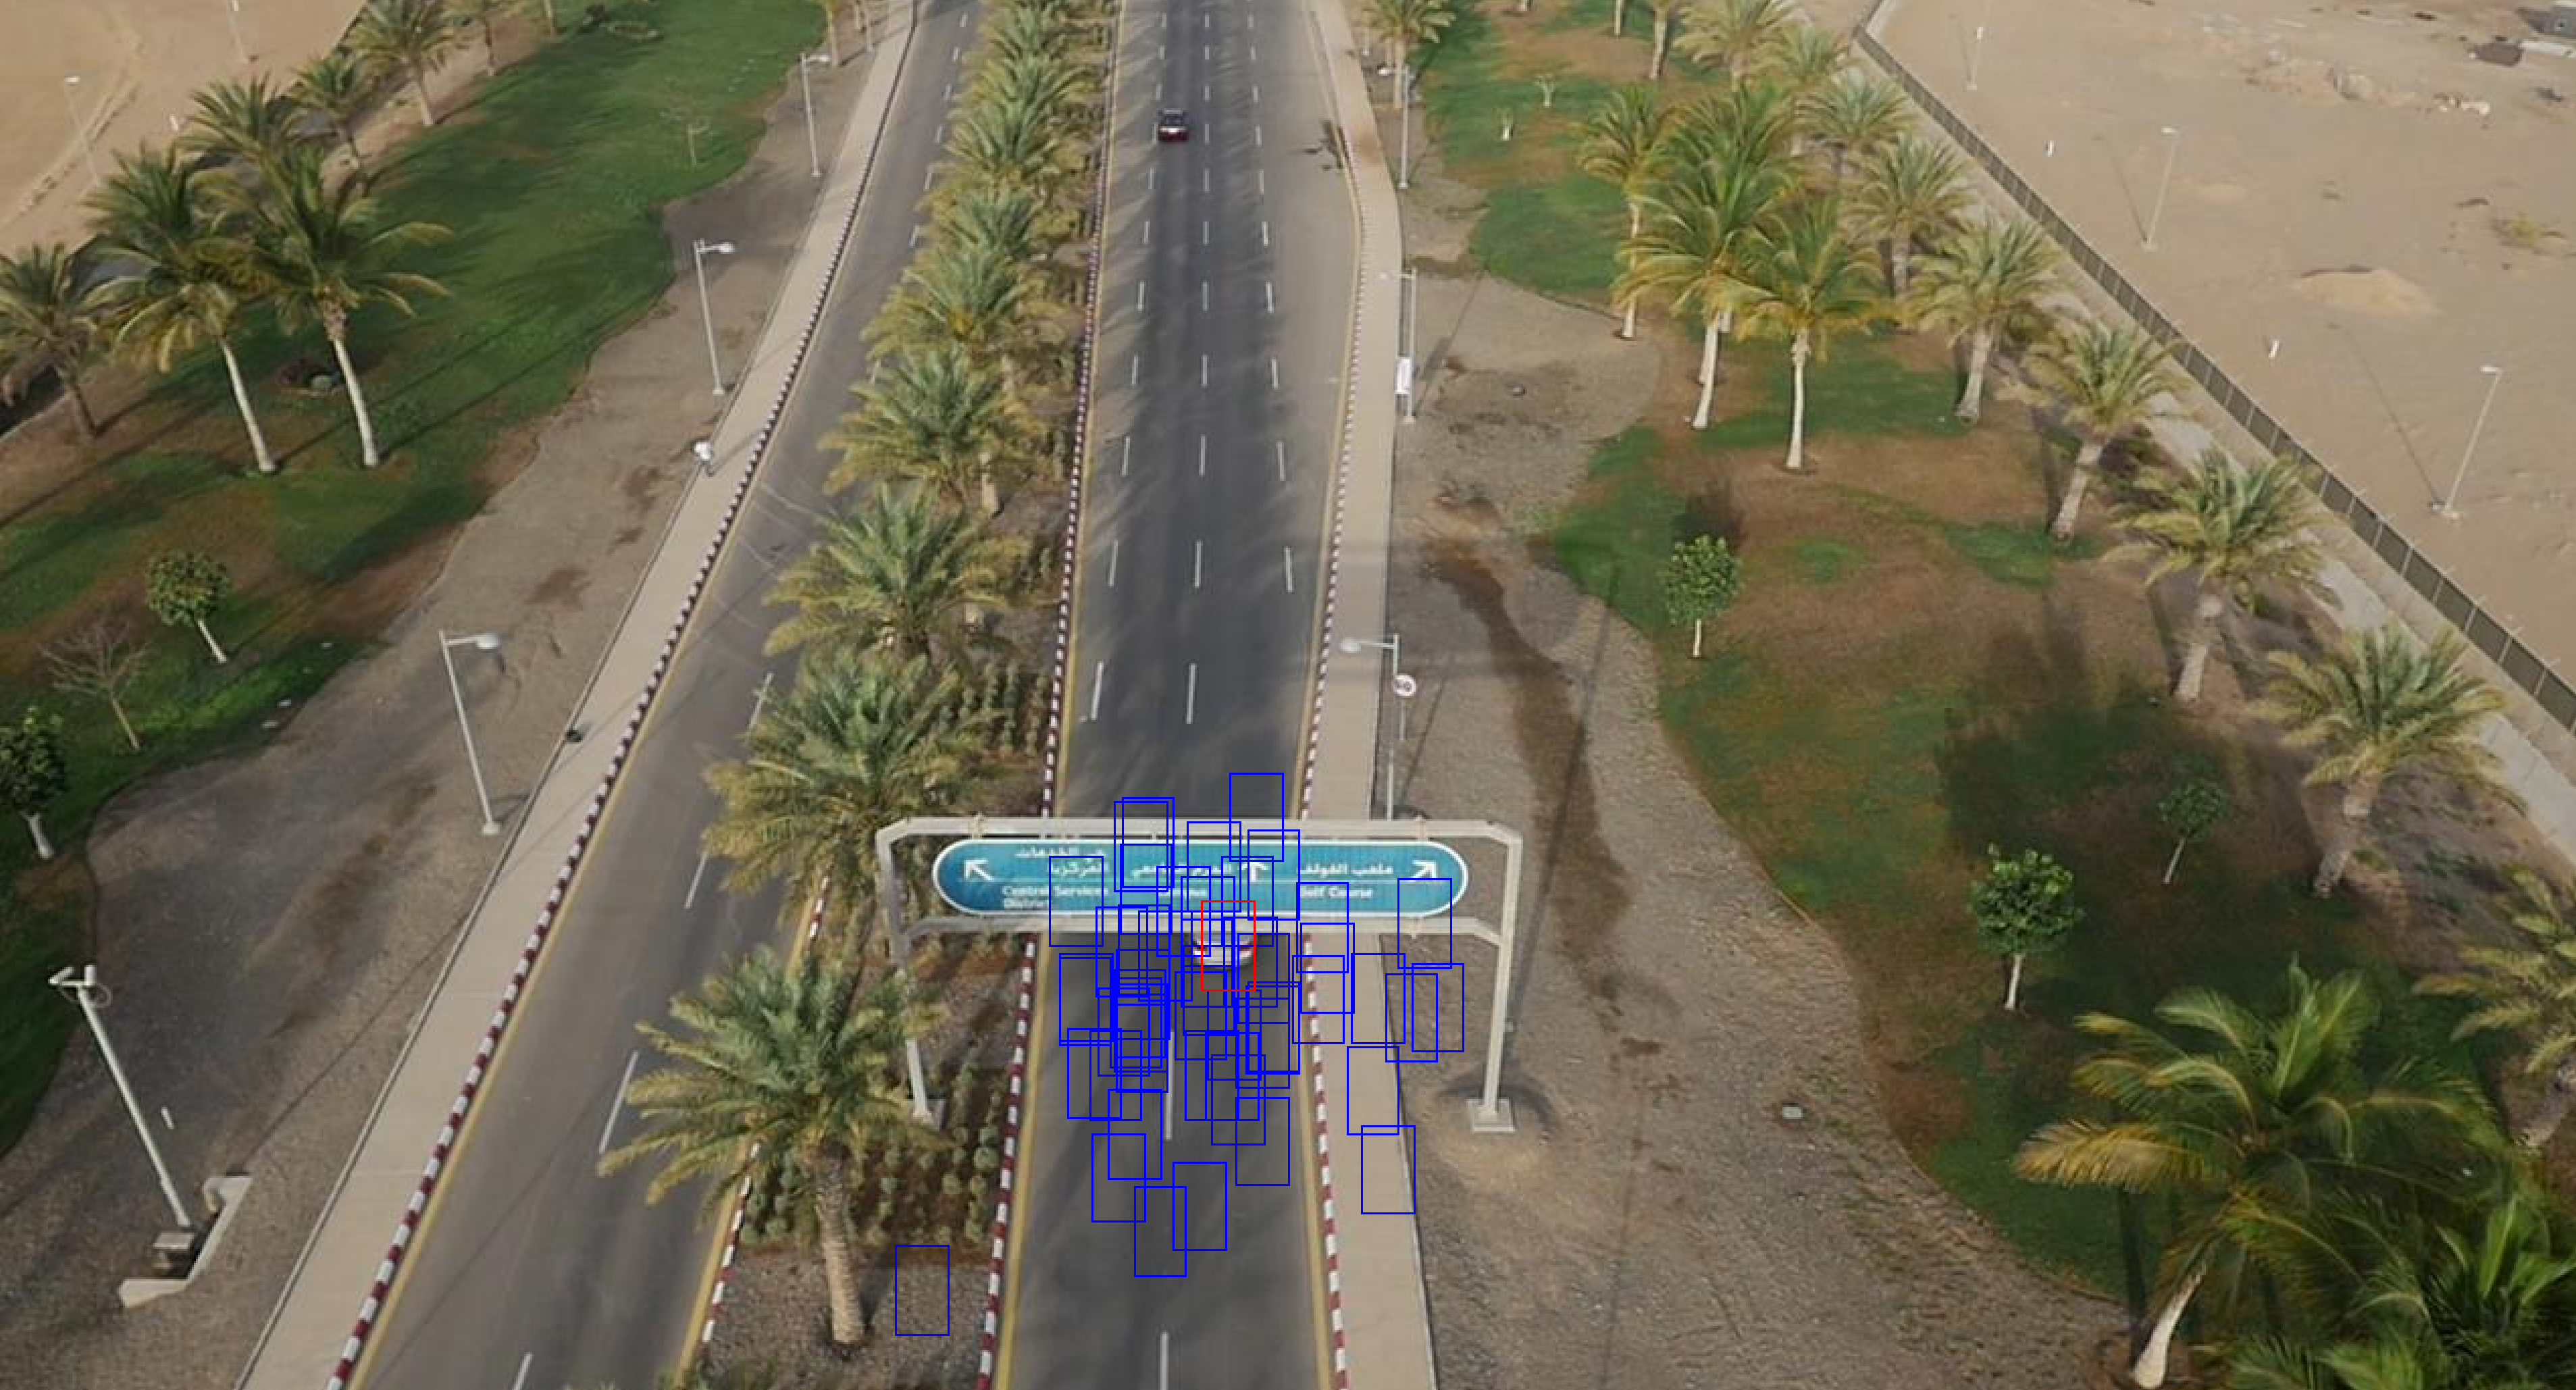
\includegraphics[width=\textwidth]{figures/gauss-pre.png}
        \caption{Sampled regions before re-detection.}
        \label{fig:sampled_before}
    \end{subfigure}
    \hfill
    \begin{subfigure}{0.25\textwidth}
        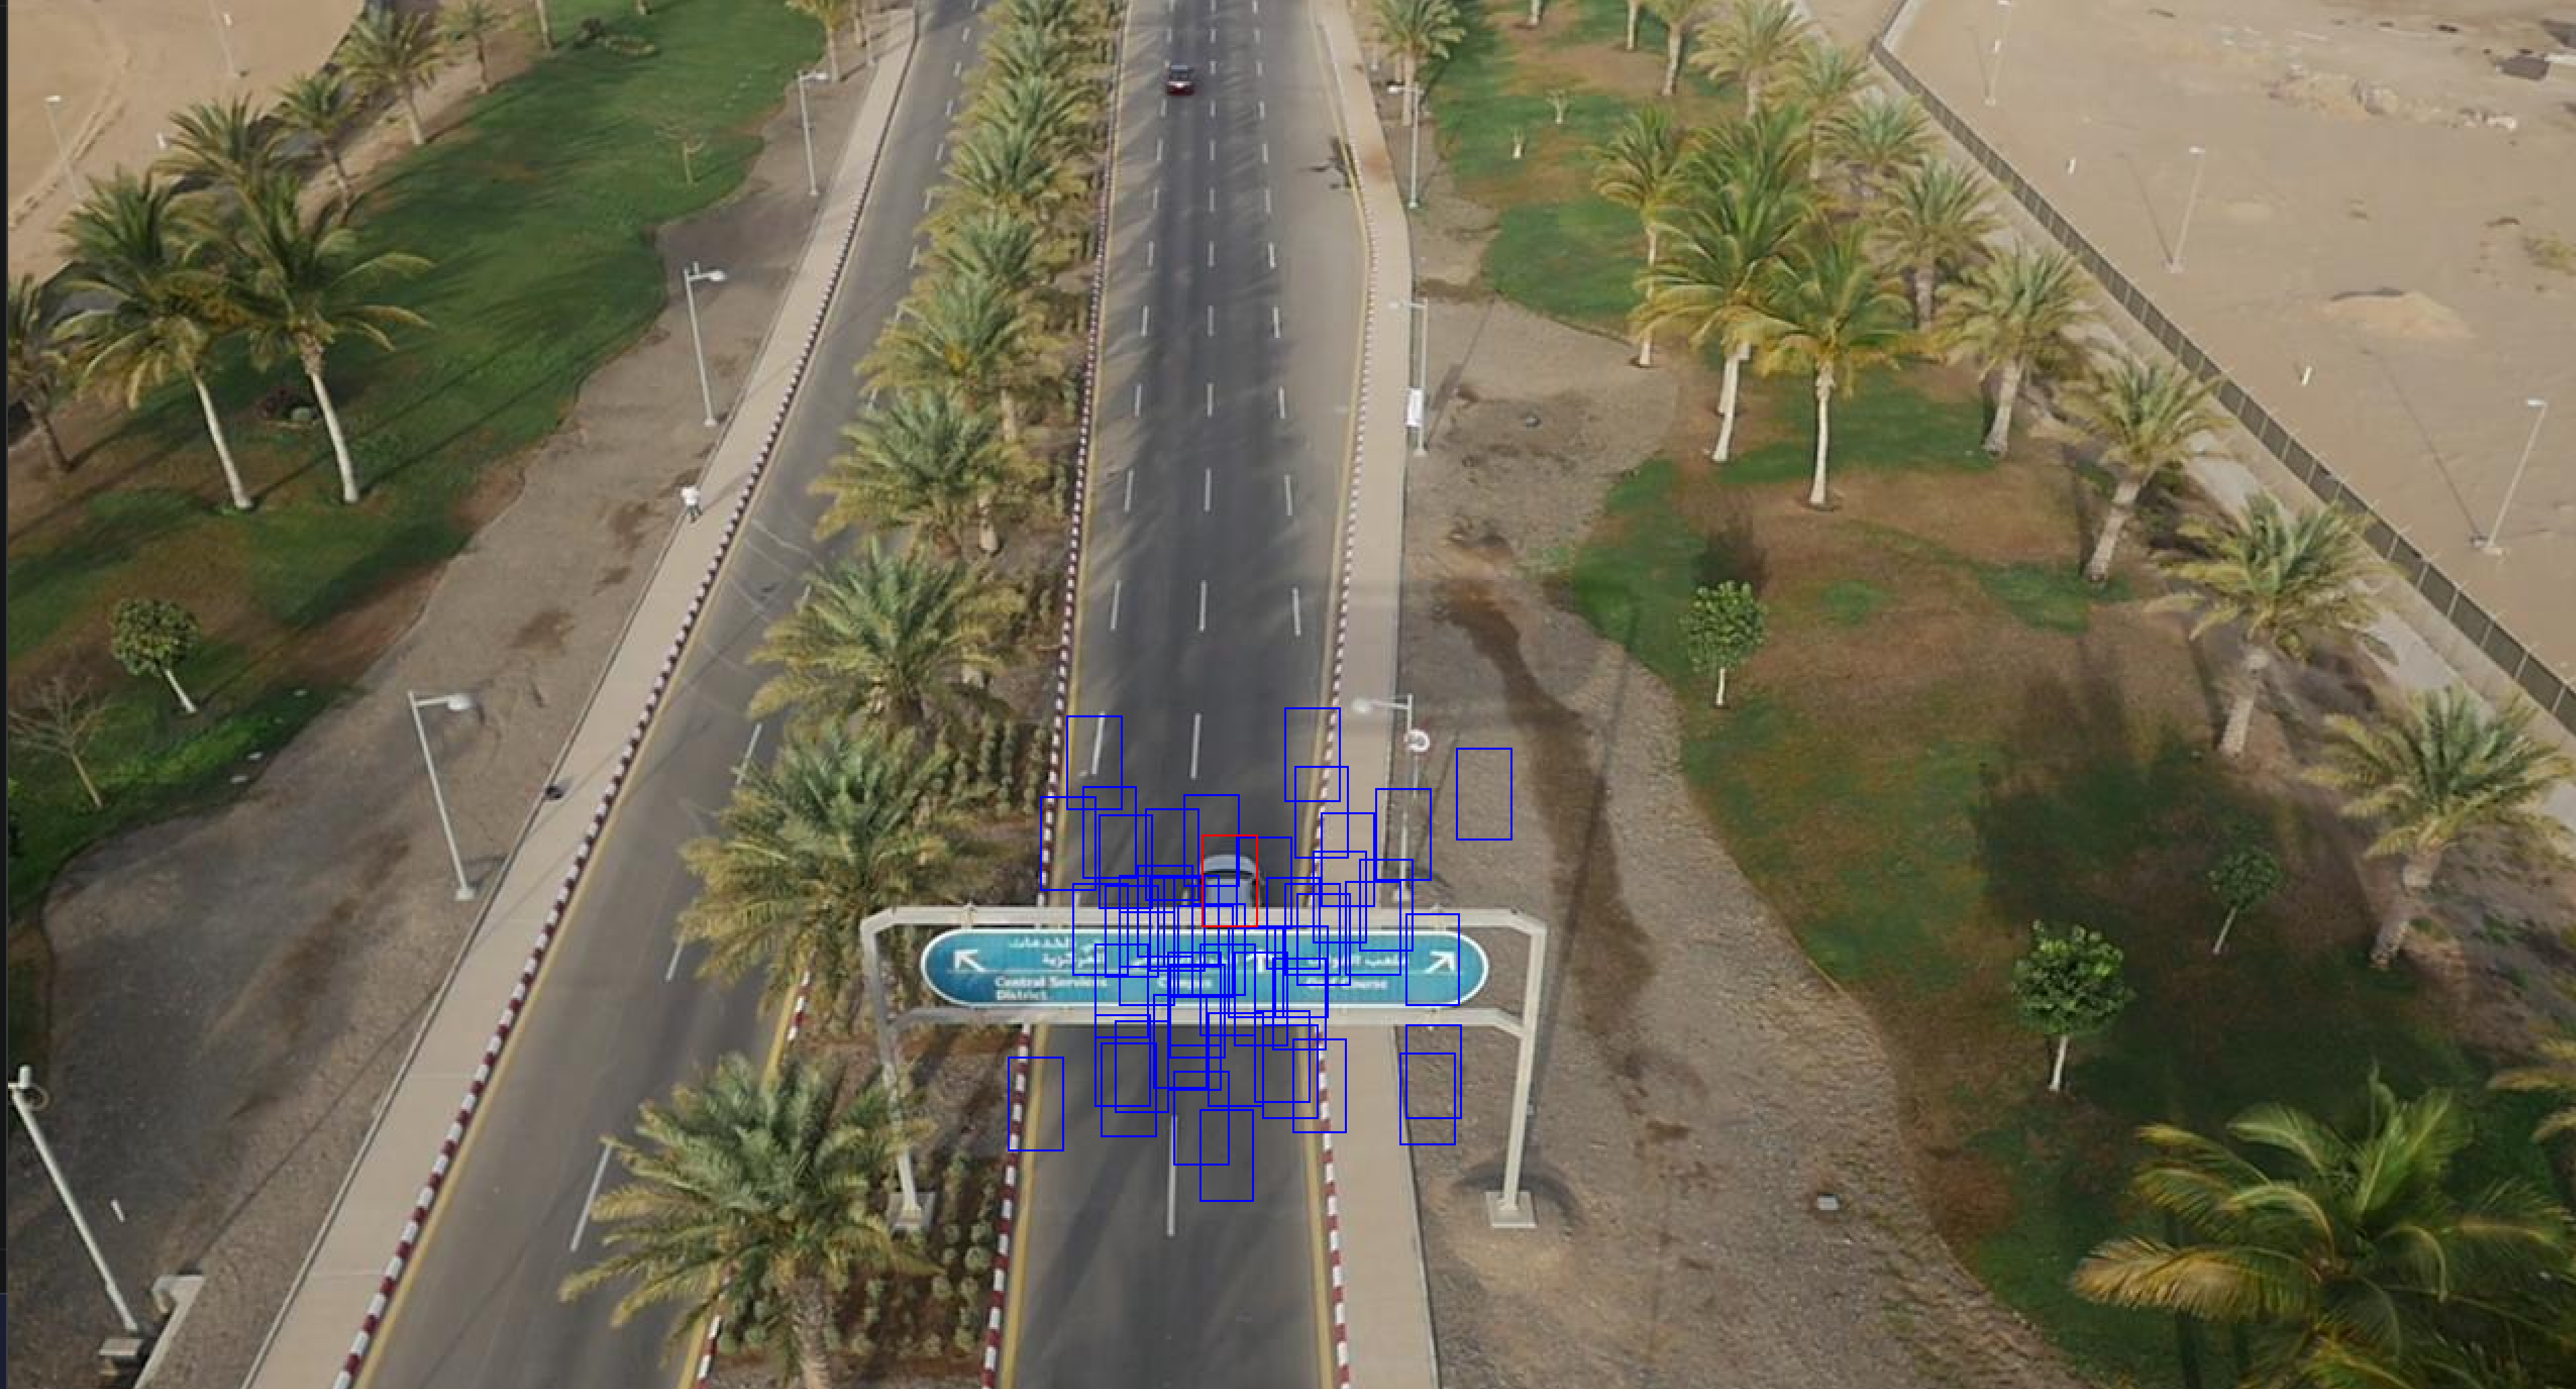
\includegraphics[width=\textwidth]{figures/gauss-post.png}
        \caption{Sampled regions after re-detection.}
        \label{fig:sampled_after}
    \end{subfigure}
    \caption{Visualization of sampled regions during re-detection with gaussian sampling.}
    \label{fig:sampled_regions:gauss:50}
\end{figure}

For example in figure~\ref{fig:sampled_regions:gauss:100} we can see that by setting $\sigma = 100$, the sampled regions
are spread wider across the image, and the detector made a similar mistake as in the uniform sampling, where it found the wrong target 
(part of the traffic sign). But after the target reappears it's able to find it again. It also takes a similar amount of frames for the target to be found again as with all the other tests done. And all the metrics
stay fairly similar as well. 

\begin{figure}[h!]
    \centering
    \begin{subfigure}[b]{0.25\textwidth}
        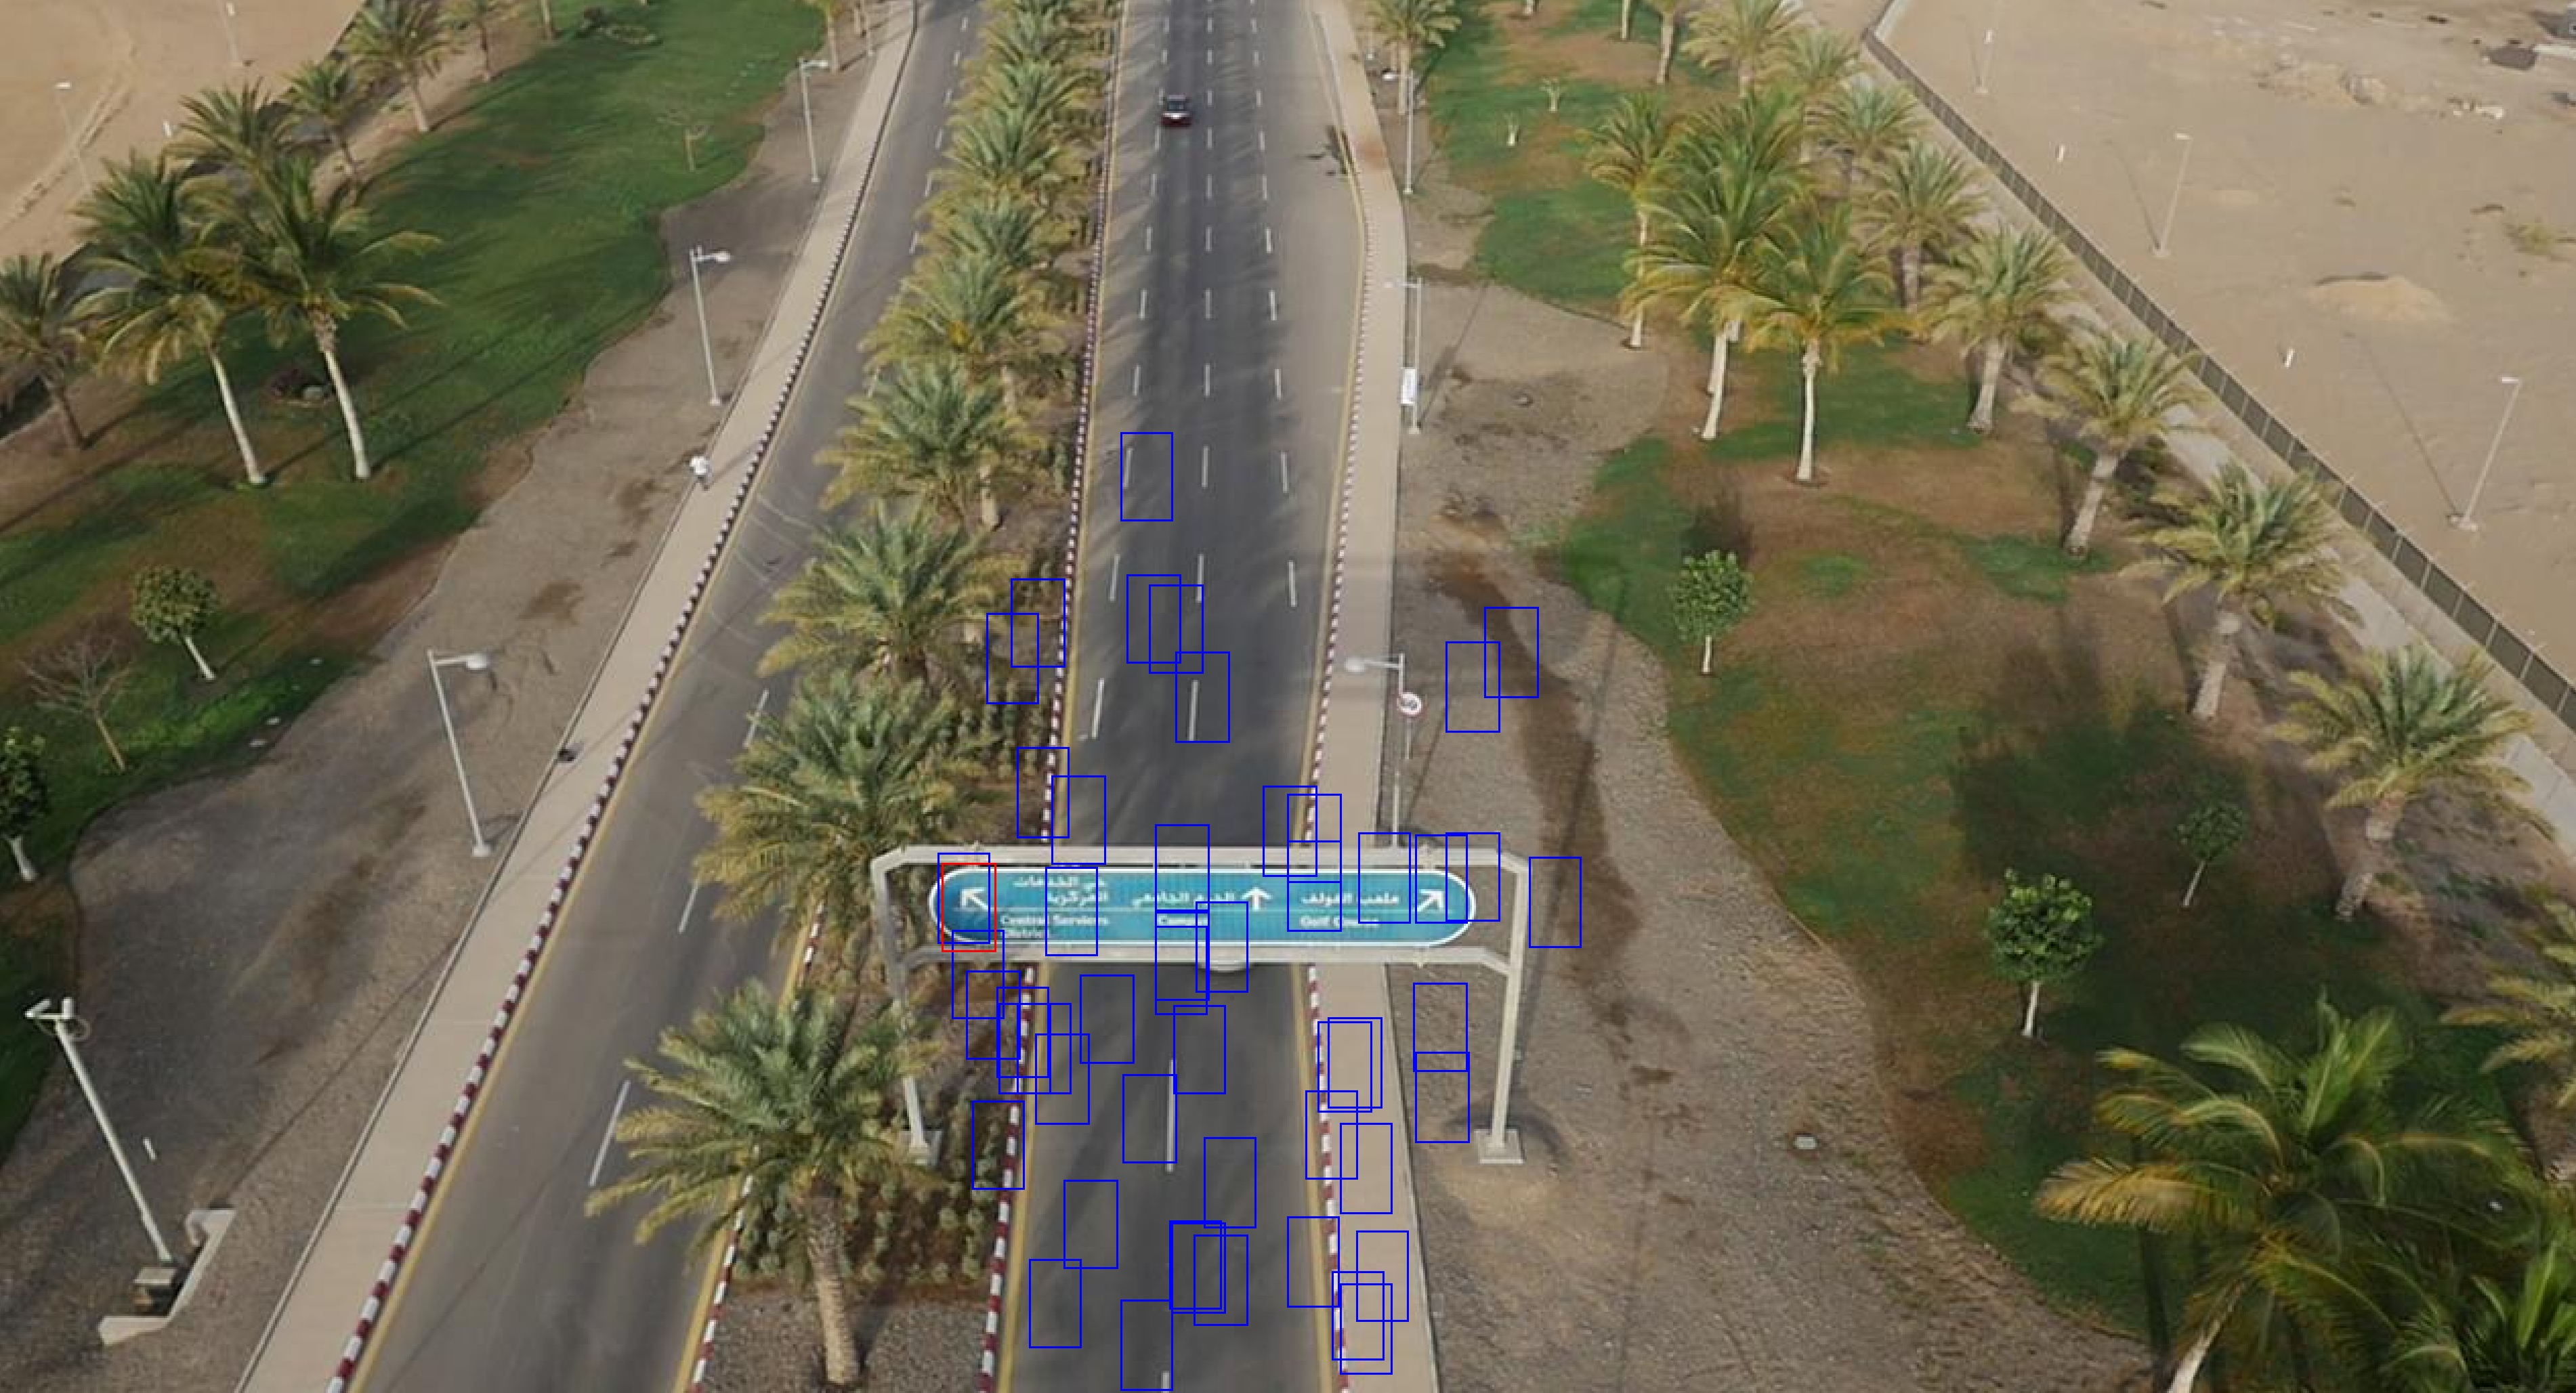
\includegraphics[width=\textwidth]{figures/gauss_100_pre.png}
        \caption{Sampled regions before re-detection.}
        \label{fig:sampled_before}
    \end{subfigure}
    \hfill
    \begin{subfigure}{0.25\textwidth}
        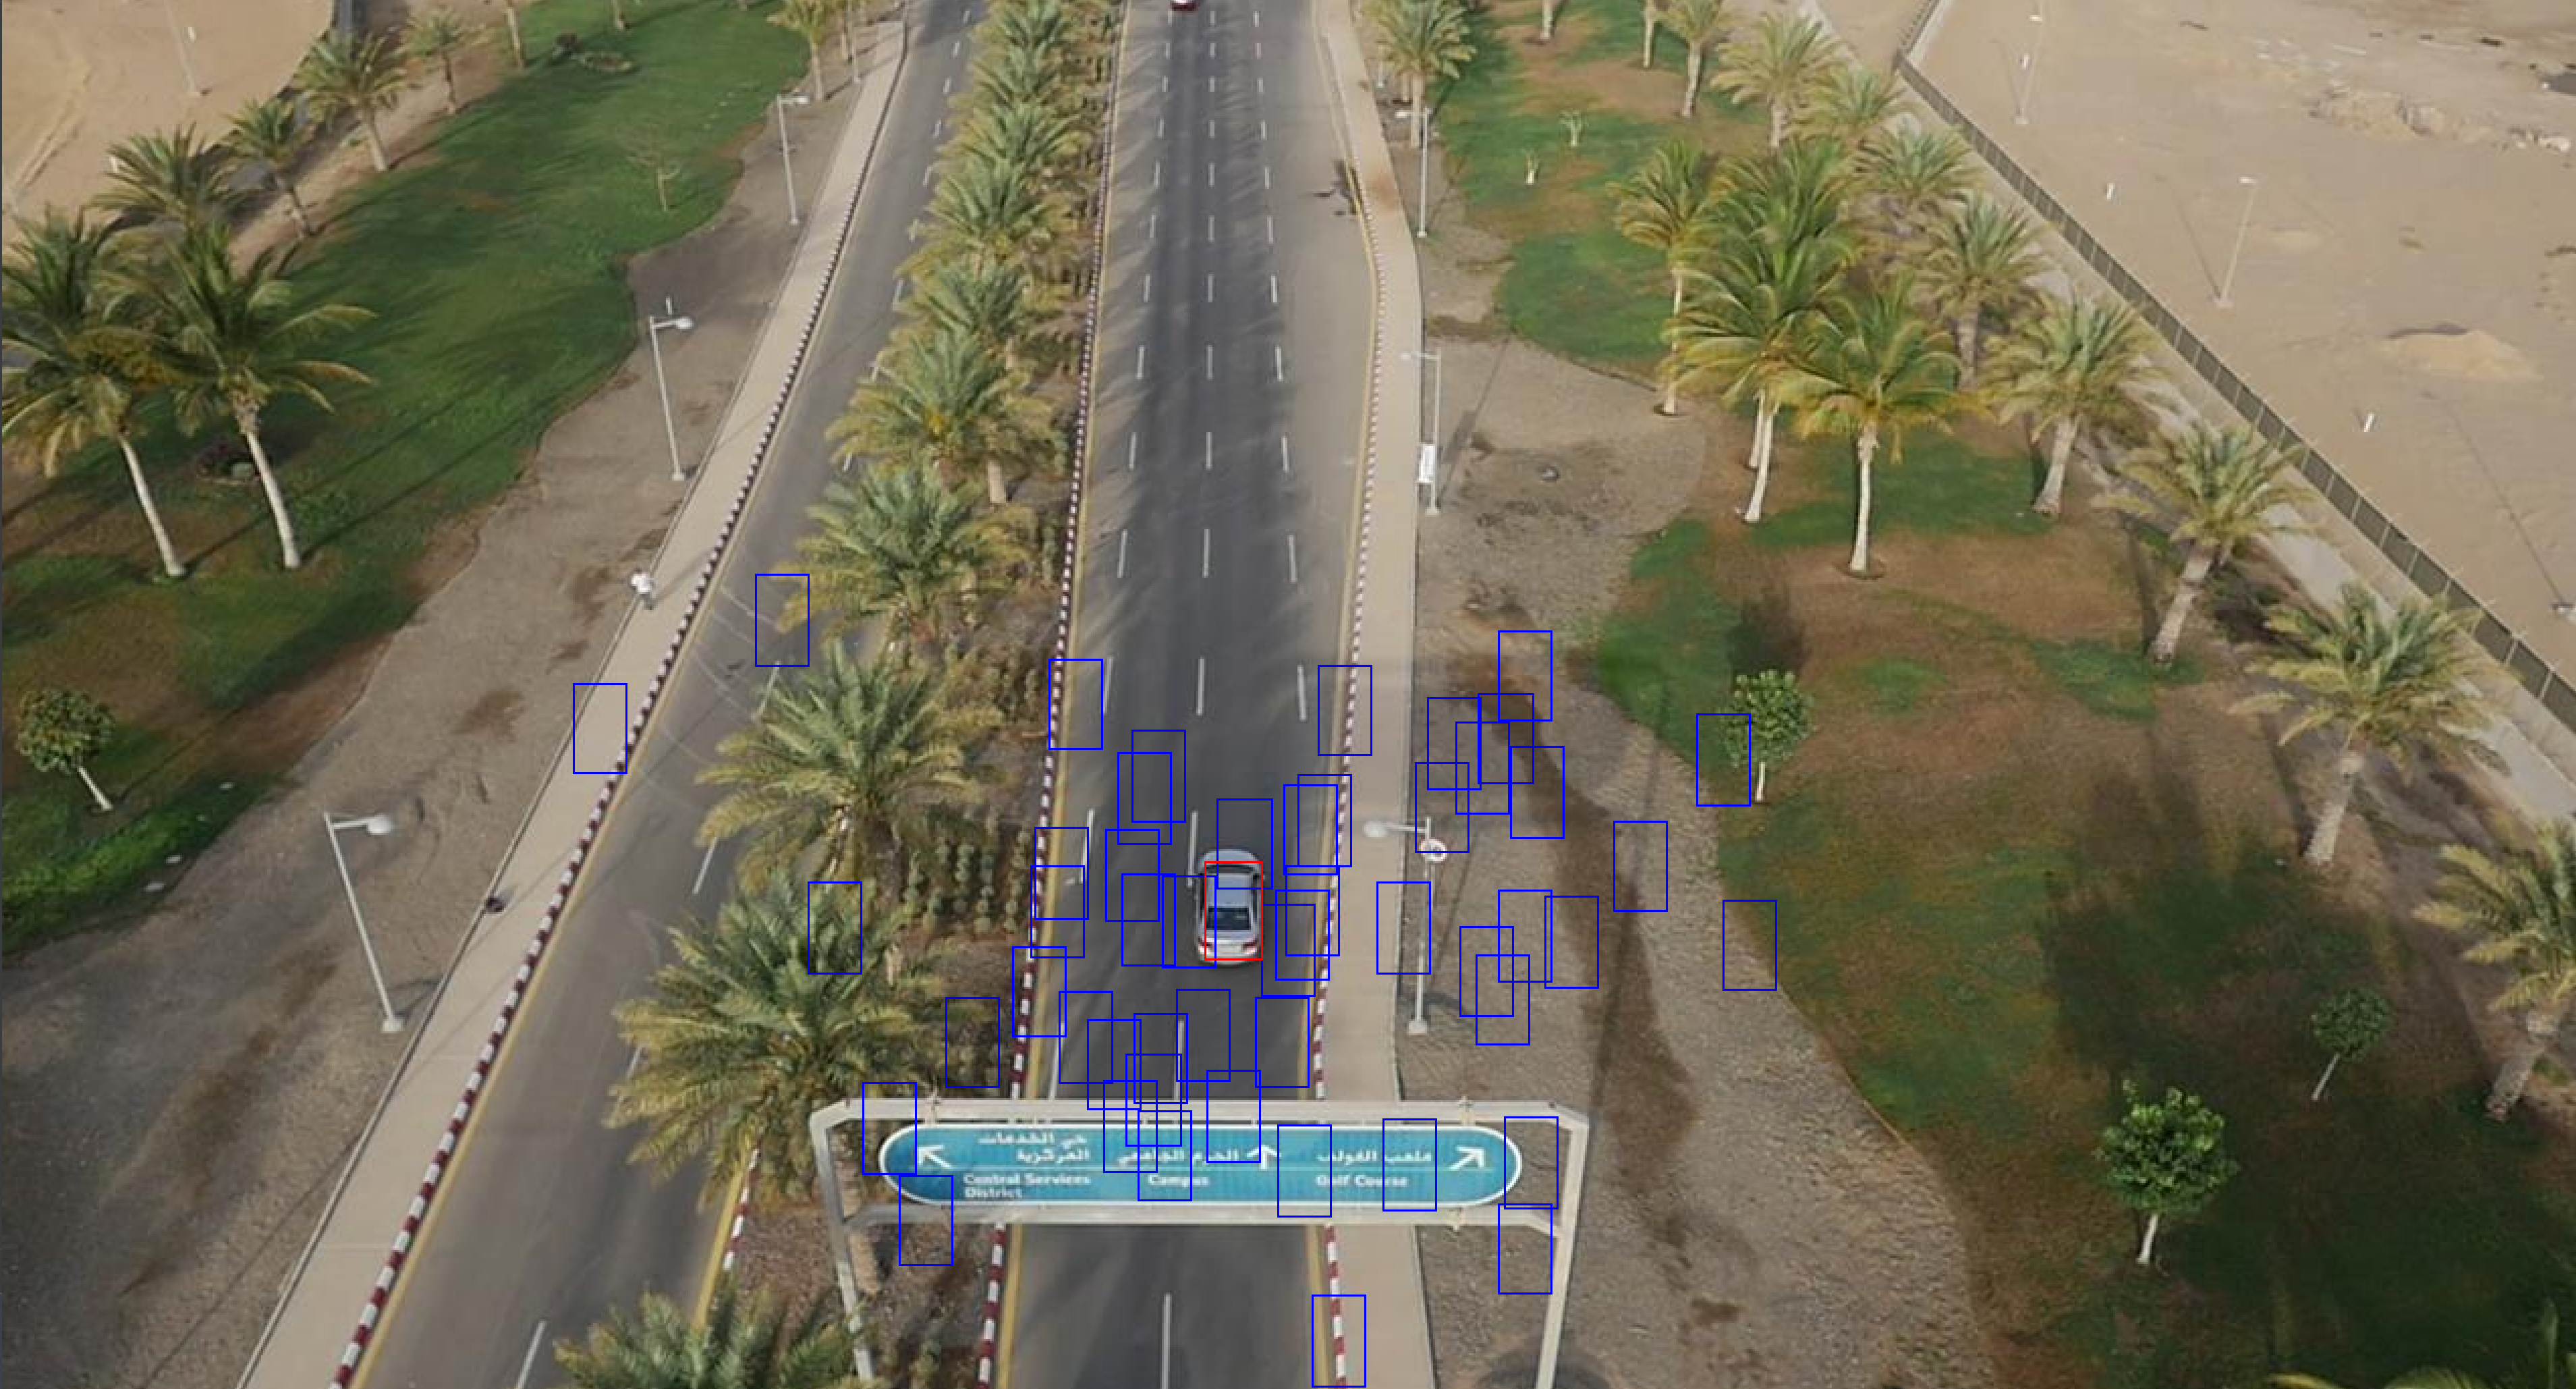
\includegraphics[width=\textwidth]{figures/gauss_100_post.png}
        \caption{Sampled regions after re-detection.}
        \label{fig:sampled_after}
    \end{subfigure}
    \caption{Visualization of sampled regions during re-detection with gaussian sampling ($\sigma = 100$).}
    \label{fig:sampled_regions:gauss:100}
\end{figure}



\section{Conclusion}

In this assignment we tested the performance of short-term tracker SiamFC on long-term sequences. We saw that the tracker
doesn't work well when and after the target disappears from view. We then adjusted the tracker to make it a long-term tracker and analyzed its
performance with different parameters. We saw that the confidence threshold is the most important parameter, when it comes to getting good
metric results. Whereas the number of sampled regions doesn't have a high effect on performance, but it does affect how fast the target
is found again after it disappears. We also tested how the tracker performs if we use gaussian sampling instead of uniform and found that the overall results
for this specific example are similar. But all the results and conclusions are based on testing only one sequence,
so they might not be generalizable to other sequences.  

\bibliographystyle{IEEEtran}
\bibliography{bibliography}

\end{document}
